\documentclass[a4paper,11pt]{article}

\usepackage[utf8]{inputenc}
\usepackage[italian]{babel}
\usepackage{graphicx}
\usepackage{subcaption}
\usepackage{csvsimple}
\graphicspath{ {images/} }
\usepackage{float}

\usepackage{geometry}
 \geometry{
 a4paper
 }
\usepackage[labelfont={bf},textfont=bf]{caption}
% settings
\usepackage{tabularx}
\usepackage{color, colortbl}
\definecolor{Gray}{gray}{0.9}
\definecolor{LightCyan}{rgb}{0.80,1,1}
\definecolor{Cyan}{rgb}{0.90,1,1}
\definecolor{LightPurple}{RGB}{219, 189, 208}
\linespread{1.1}
 \renewcommand{\labelitemi}{$\textendash$}

 \setlength{\parindent}{0ex}

\begin{document}

\author{Giulia Cantini}
\title{A Tandem Queueing Model for Delay Analysis in Disconnected Ad Hoc Networks\\
\vspace{0.5cm}
\Large{An OMNeT++ simulation}}
\maketitle
\date

\tableofcontents

\section{Introduzione}
I tradizionali protocolli di routing \textit{store-and-forward}, che richiedono l'esistenza di un cammino
end-to-end che colleghi sorgente e destinazione, non possono essere utilizzati in reti
soggette a disconnessioni frequenti. Una soluzione che può risolvere questo problema è
sfruttare il movimento dei nodi della rete ed utilizzare il paradigma \textit{store-carry-and-forward}.

In tali reti, chiamate \textit{Delay Tolerant Networks} (DTN), il ritardo di trasmissione dei dati tra i nodi
può risultare elevato a causa delle disconnessioni.

Un importante fattore che caratterizza le DTN è l'opportunità di contatto tra coppie di nodi.
Due nodi sono in contatto se si trovano entro il range di trasmissione l'uno dell'altro,
ovvero ad una distanza tale da consentire lo scambio di pacchetti.

Il modello sviluppato consiste di una rete opportunistica formata da un insieme di tre code
che collaborano tra loro per realizzare il meccanismo opportunistico.

Esso si basa sulle seguenti assunzioni:

\begin{enumerate}
  \item I contatti sono puramente opportunistici, ovvero non si ha nessuna conoscenza
  di quando questi avverranno (protocollo \textit{no-context});
  \item la distribuzione dei tempi di inter-contatto ha media e varianza finite;
  \item il nodo sorgente ha in arrivo un flusso di pacchetti;
  \item i nodi sorgente e destinazione sono fissi, mentre i nodi intermedi sono mobili e
  fungono da \textit{relay};
  \item il modello è basato su due code che sono servite in alternanza da un singolo server.
  Il server è autonomo e non c'è modo di controllarne il movimento;
  \item il nodo mobile salva i pacchetti che provengono dalla sorgente e li inoltra a destinazione;
  \item il nodo mobile non è mai nel \textit{range} di sorgente e destinazione allo stesso tempo.

\end{enumerate}

\section{Modello}

Il modello considerato consiste di 3 sistemi a server singolo first-in-first-out (FIFO) con coda a capacità illimitata, \textit{Q\textsubscript{i}}, i = 1,2,3 in cui i pacchetti arrivano in \textit{Q\textsubscript{1}} e successivamente richiedono il servizio in \textit{Q\textsubscript{2}} prima di raggiungere la destinazione in \textit{Q\textsubscript{3}}. 
Particolare caratteristica del modello è che \textit{Q\textsubscript{2}} si alterna tra le posizioni \textit{L\textsubscript{1}} e \textit{L\textsubscript{2}} in modo che il server di \textit{Q\textsubscript{1}} è disponibile solamente quando \textit{Q\textsubscript{2}} si trova in \textit{L\textsubscript{1}} e il server di \textit{Q\textsubscript{2}} è disponibile solo quando \textit{Q\textsubscript{2}} si trova in \textit{L\textsubscript{2}}. \newline
Inoltre esiste un tempo di \textit{switch-over} da \textit{L\textsubscript{i}} a \textit{L\textsubscript{j}} $(\textit{i} \neq \textit{j},  \textit{j} \in \{1,2\})$
in cui né il server in \textit{Q\textsubscript{1}} né il server in \textit{Q\textsubscript{2}} sono disponibili.\newline
\textit{Q\textsubscript{3}} funge da \textit{sink} e non viene considerata nell'analisi. \newline
\textit{Q\textsubscript{2}} si muove in maniera autonoma, rimanendo in una determinata locazione L per un intervallo di tempo generato da una distribuzione esponenziale (\textit{tempo di permanenza}).\newline
Durante il periodo di disponibilità di un server in \textit{Q\textsubscript{1}} o \textit{Q\textsubscript{2}}, questo può alternare momenti di servizio e momenti in cui è \textit{idle}, in base alla presenza di clienti/pacchetti da servire.

\begin{figure}[h!]
    \centering
    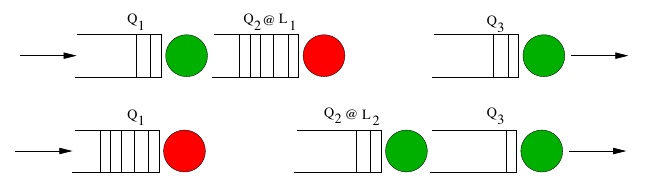
\includegraphics[width=\linewidth]{images/oppnet-model.png}
    \caption{Modello a tre code con una coda mobile.
    Top: Quando \textit{Q\textsubscript{2}} è in \textit{L\textsubscript{1}}, il suo server è down.
    Bottom: Quando \textit{Q\textsubscript{2}} è in \textit{L\textsubscript{2}}, il suo server è up.}
    \label{fig:1}
\end{figure}
\newpage
\section{Implementazione}

Nella rete modellata, denominata \textit{OppNet}, \textit{Q\textsubscript{1}} e \textit{Q\textsubscript{2}} sono due moduli \textit{OppPassiveQueue} serviti da un unico server \textit{S}, \textit{Q\textsubscript{3}} è una coda con server built-in, e sono presenti inoltre una \textit{source} che genera i pacchetti e un \textit{sink} che li raccoglie dopo che hanno attraversato l'intero sistema.\newline

\begin{figure}[h!]
    \centering
    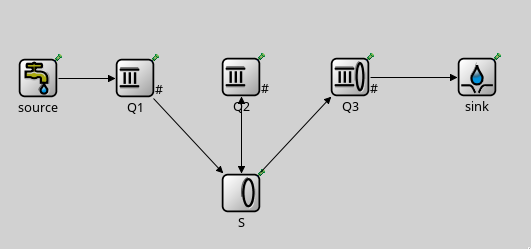
\includegraphics[width=\linewidth]{images/oppnet-mymodel.png}
    \caption{Visualizzazione del file oppnet.ned}
    \label{fig:2}
\end{figure}

Il comportamento di \textit{S} è determinato dalla classe OppServer.cc che estende la classe \textit{Server} presente nella libreria \textit{queueinglib}.\newline
Il meccanismo opportunistico è implementato introducendo due nuovi tipi di eventi: \textit{startSwitchEvent} e \textit{endSwitchOverTimeEvent}, che delimitano il periodo di \textit{switch over}, in cui il server non è disponibile per nessuna delle due code: il primo si verifica per segnalare l'inizio dello \textit{switch} ed il secondo per segnalarne la fine.\newline
La non disponibilità del server è espressa dalla variabile booleana \textit{serverIsAvailable}.\newline
Un'altra \textit{flag} \textit{isServingQ1} viene invece utilizzata per controllare quale coda tra \textit{Q\textsubscript{1}} e \textit{Q\textsubscript{2}} deve essere servita.

\begin{figure}[h!]
    \centering
    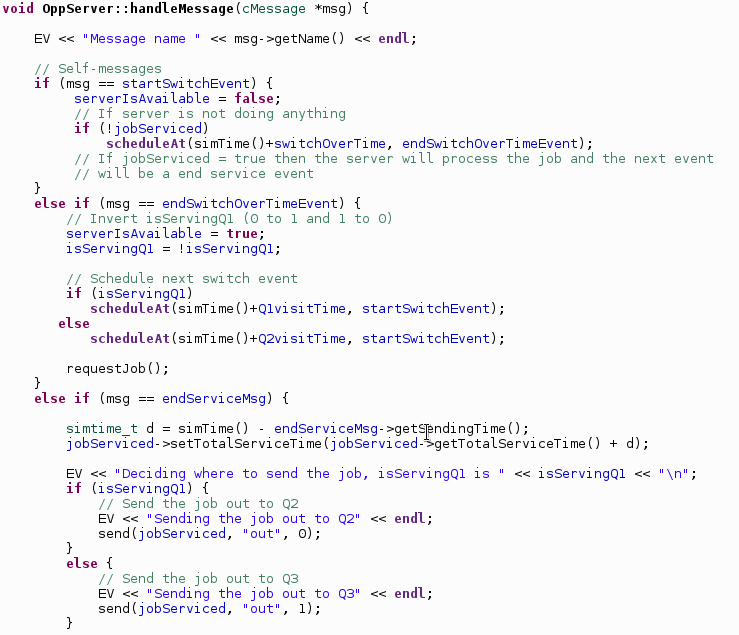
\includegraphics[width=\linewidth]{images/handle-message-oppserver.png}
    \caption{Gestione dello \textit{switch over} e alternanza del server tra le due code \textit{Q\textit{1}} e \textit{Q\textsubscript{2}}.}
    \label{fig:1}
\end{figure}
\newpage
\section{Simulazione}

% eseguire la simulazione da riga di comando
% ./oppnet-sim -m -n .:../../Scaricati/omnetpp-5.4/samples/queueinglib -l ../../Scaricati/omnetpp-5.4/samples/queueinglib/queueinglib omnetpp.ini -c PreliminarySimulation 

\subsection{Misure di prestazione}
Le variabili di interesse considerate per la simulazione sono state:
\begin{itemize}
    \item Tempo medio di risposta del sistema, ovvero il tempo medio di soggiorno dell'utente (\textit{pacchetto}) nel sistema, dalla generazione nella \textit{source} all'arrivo nel \textit{sink}.
    \item Numero medio di utenti in coda nel sistema, di cui si è analizzato singolarmente la media delle lunghezze delle tre code \textit{Q\textsubscript{1}}, \textit{Q\textsubscript{2}}, \textit{Q\textsubscript{3}}.
    \item Throughput medio del sistema, ovvero la media di utenti serviti sull'intervallo di tempo.
\end{itemize}
La simulazione è stata parametrizzata in base al processo di arrivo dei pacchetti nel sistema, esponenziale di media {5s, 7.5s, 10s}.
\subsection{Transiente iniziale}
In una simulazione stazionaria si è interessati ad analizzare il comportamento del modello nello \textit{stato stazionario}, raggiunto quando le variabili di interesse iniziano a presentare regolarità statistica. Il periodo antecedente a questo stato è denominato \textit{transiente iniziale} o \textit{warm-up period}. \newline
Per determinare questo intervallo di tempo si è eseguita inizialmente una simulazione preliminare relativamente lunga (\textit{1h}, lunghezza determinata tramite prove ripetute), su tre \textit{run} independenti per parametro, misurando lunghezze delle tre code, tempo di soggiorno e throughput sia per singole \textit{run} che per \textit{averaged}.\newline
Nelle pagine che seguono sono riportati alcuni grafici ottenuti tramite analisi con lo script R \textit{estimate\_warmup} e utilizzati per la stima del transiente.\newline
I grafici in questione riportano in modo puntuale lunghezze di \textit{Q\textsubscript{1}}, \textit{Q\textsubscript{2}}, \textit{Q\textsubscript{3}}, tempo di risposta del sistema e throughput del sistema, dove ogni punto è risultato della media delle tre \textit{run}.
\newpage
%%%%% LUNGHEZZA DI Q1 
\begin{figure}[h!]
    \begin{subfigure}[t]{.5\textwidth}
      \centering
      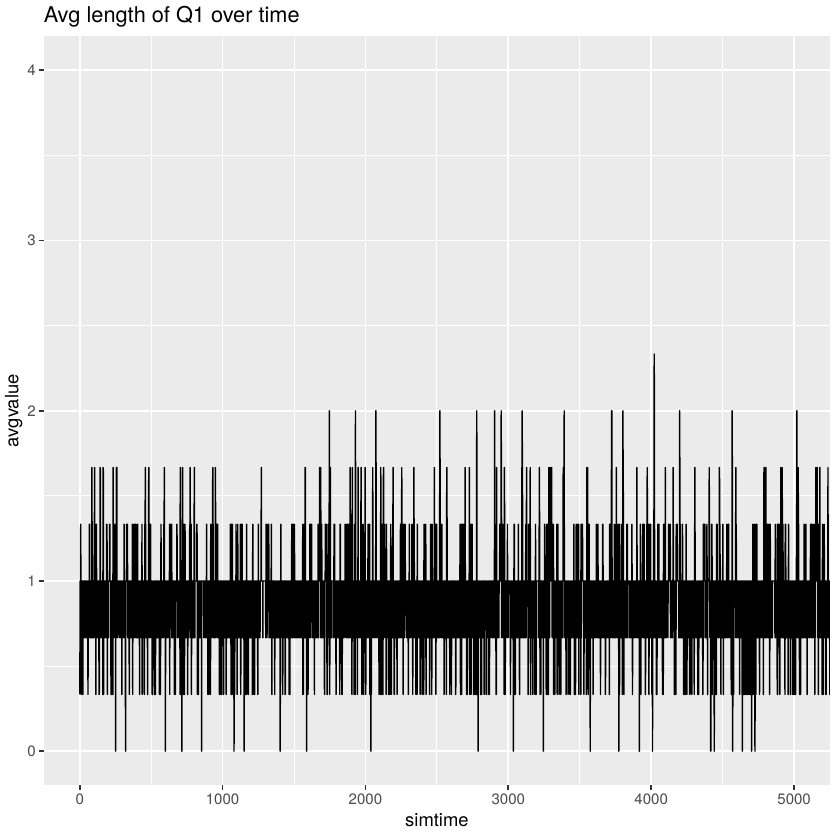
\includegraphics[width=.9\linewidth]{images/chart-q1avglength-5.png}
      \caption{p = 5s}
      \label{fig:sfig1}
    \end{subfigure}%
    \begin{subfigure}[t]{.5\textwidth}
      \centering
      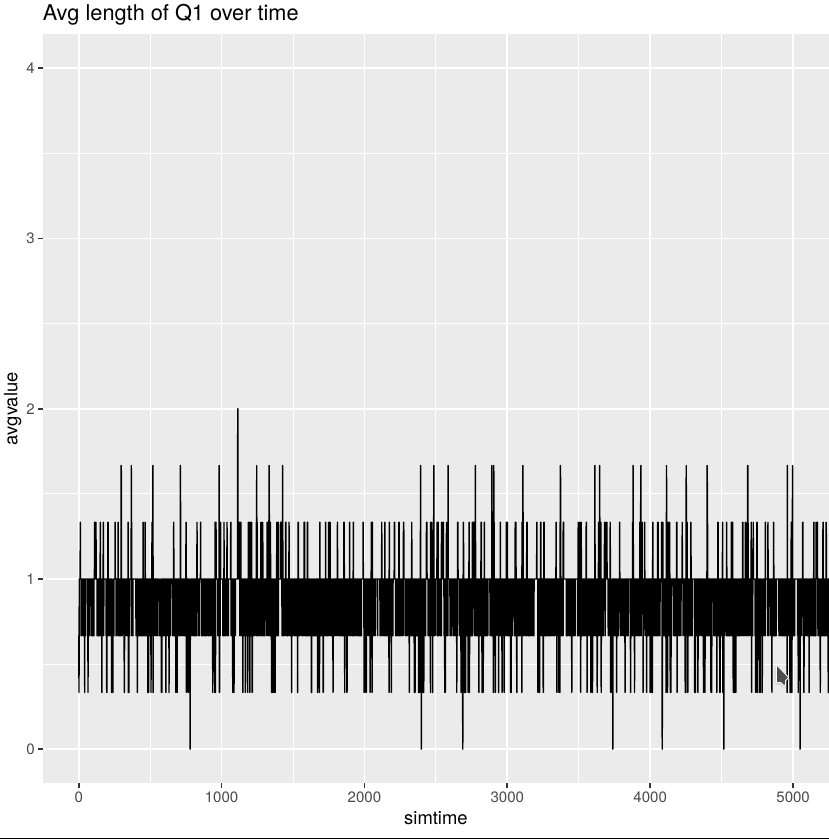
\includegraphics[width=.9\linewidth]{images/chart-q1avglength-75.png}
      \caption{p = 7.5s}
      \label{fig:sfig2}
    \end{subfigure}
    \begin{subfigure}[t]{\textwidth}
      \centering
      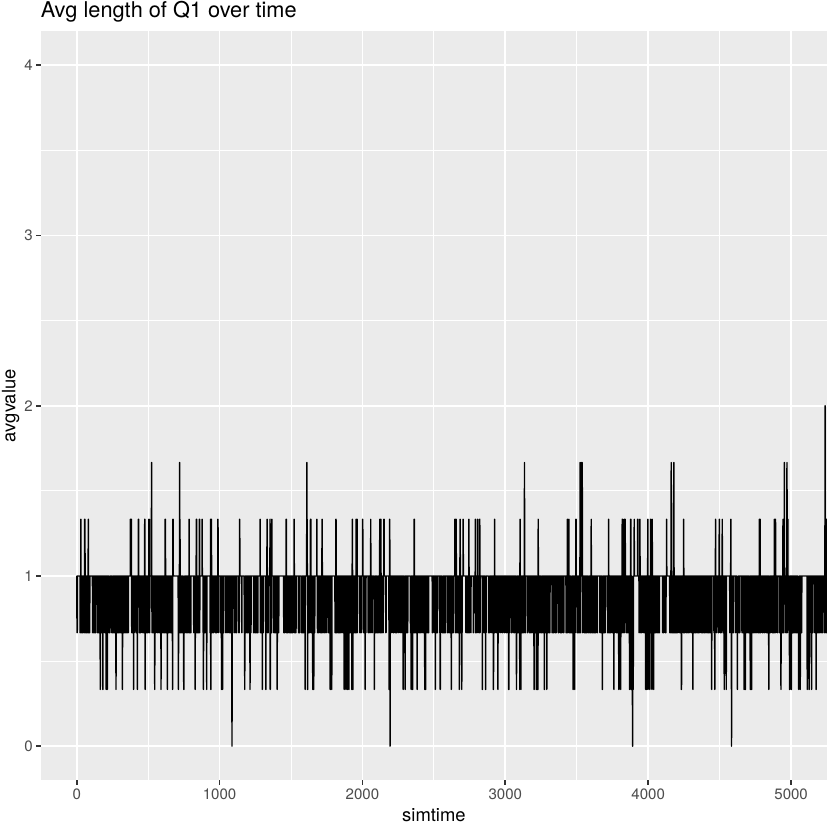
\includegraphics[width=.45\linewidth]{images/chart-q1avglength-10.png}
      \caption{p = 10s}
      \label{fig:sfig2}
    \end{subfigure}
    \caption{Lunghezza di \textit{Q\textsubscript{1}} per i tre rispettivi tempi di interarrivo \textit{p}}
    \label{fig:fig}
\end{figure}
\newpage

%%%%% LUNGHEZZA DI Q2
\begin{figure}[h!]
\begin{subfigure}{.5\textwidth}
  \centering
  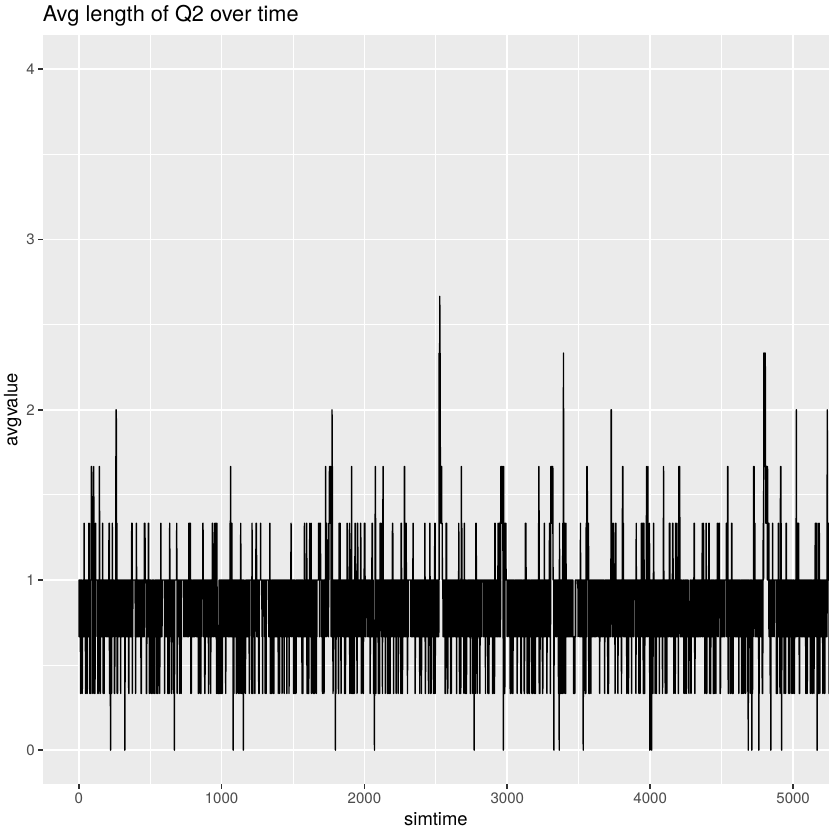
\includegraphics[width=.9\linewidth]{images/chart-q2avglength-5.png}
  \caption{p = 5s}
  \label{fig:sfig1}
\end{subfigure}%
\begin{subfigure}{.5\textwidth}
  \centering
  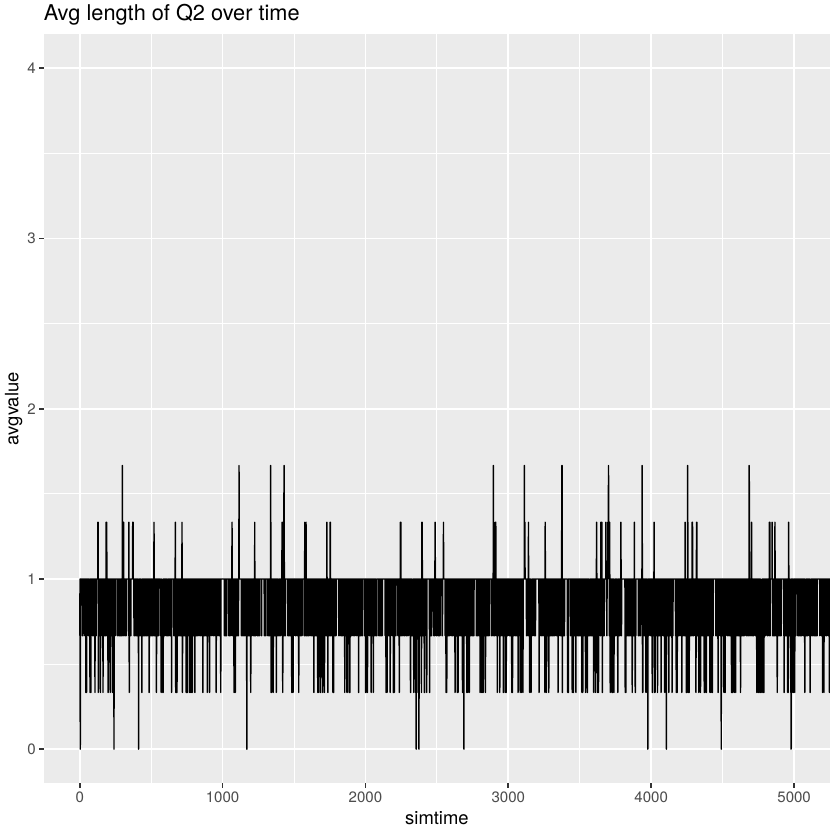
\includegraphics[width=.9\linewidth]{images/chart-q2avglength-75.png}
  \caption{p = 7.5s}
  \label{fig:sfig2}
\end{subfigure}
\begin{subfigure}{\textwidth}
  \centering
  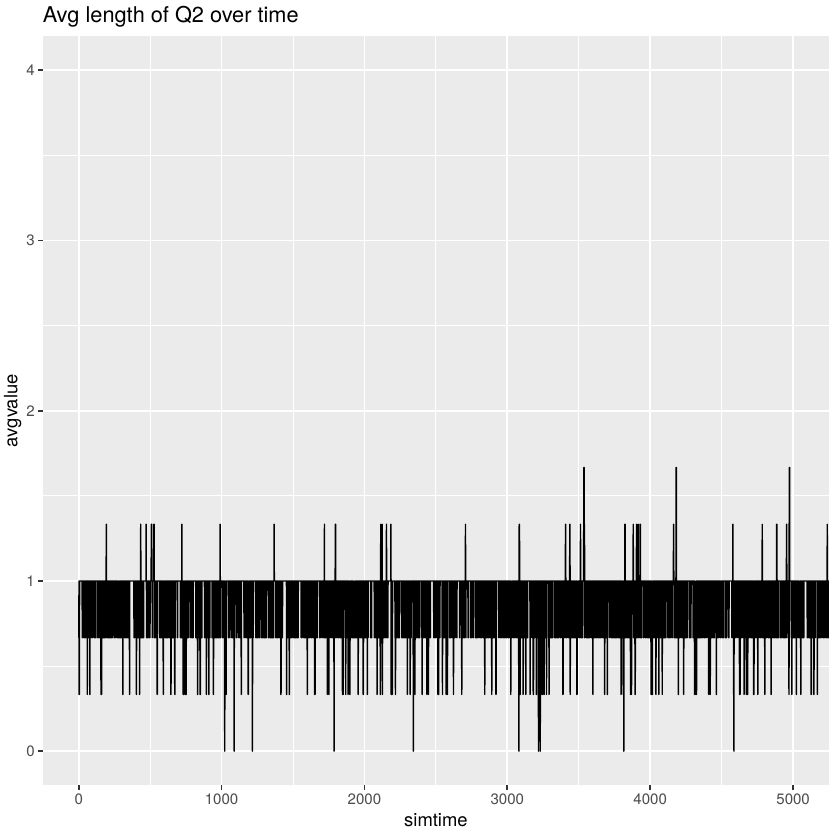
\includegraphics[width=.45\linewidth]{images/chart-q2avglength-10.png}
  \caption{p = 10s}
  \label{fig:sfig2}
\end{subfigure}
\caption{Lunghezza di \textit{Q\textsubscript{2}} per i tre rispettivi tempi di interarrivo \textit{p}}
\label{fig:fig}
\end{figure}
\newpage
%%% LUNGHEZZA DI Q3
\begin{figure}[h!]
\begin{subfigure}{.5\textwidth}
  \centering
  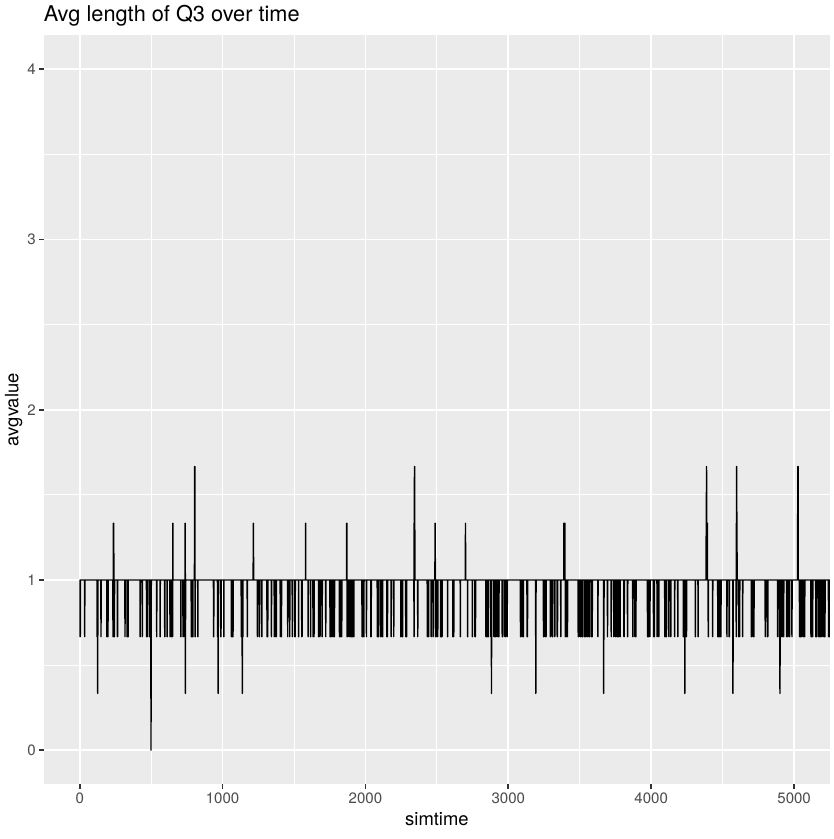
\includegraphics[width=.9\linewidth]{images/chart-q3avglength-5.png}
  \caption{p = 5s}
  \label{fig:sfig1}
\end{subfigure}%
\begin{subfigure}{.5\textwidth}
  \centering
  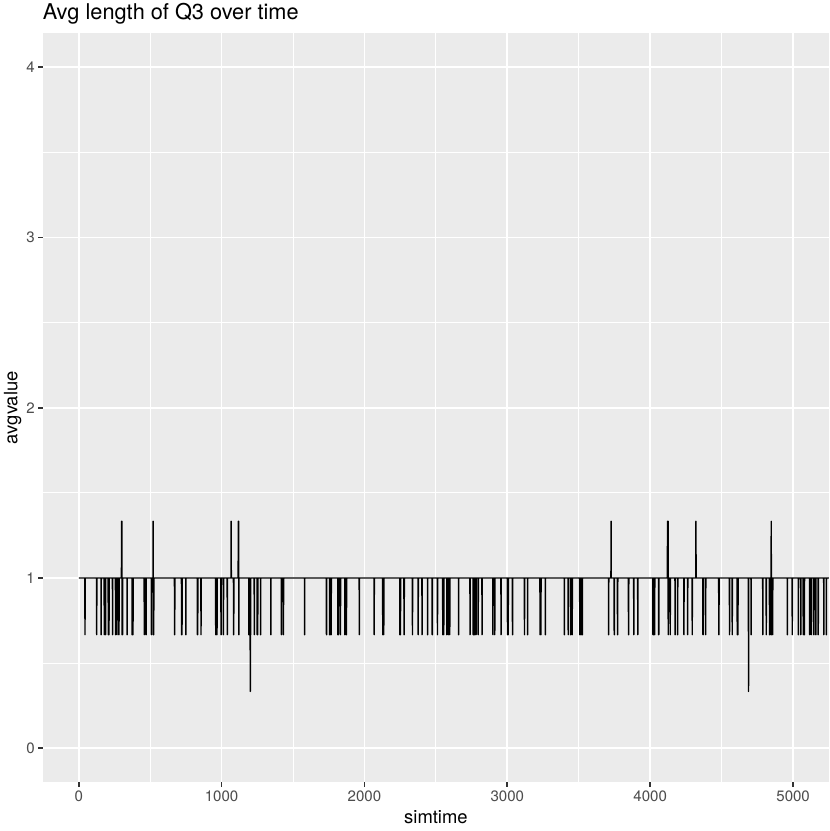
\includegraphics[width=.9\linewidth]{images/chart-q3avglength-75.png}
  \caption{p = 7.5s}
  \label{fig:sfig2}
\end{subfigure}
\begin{subfigure}{\textwidth}
  \centering
  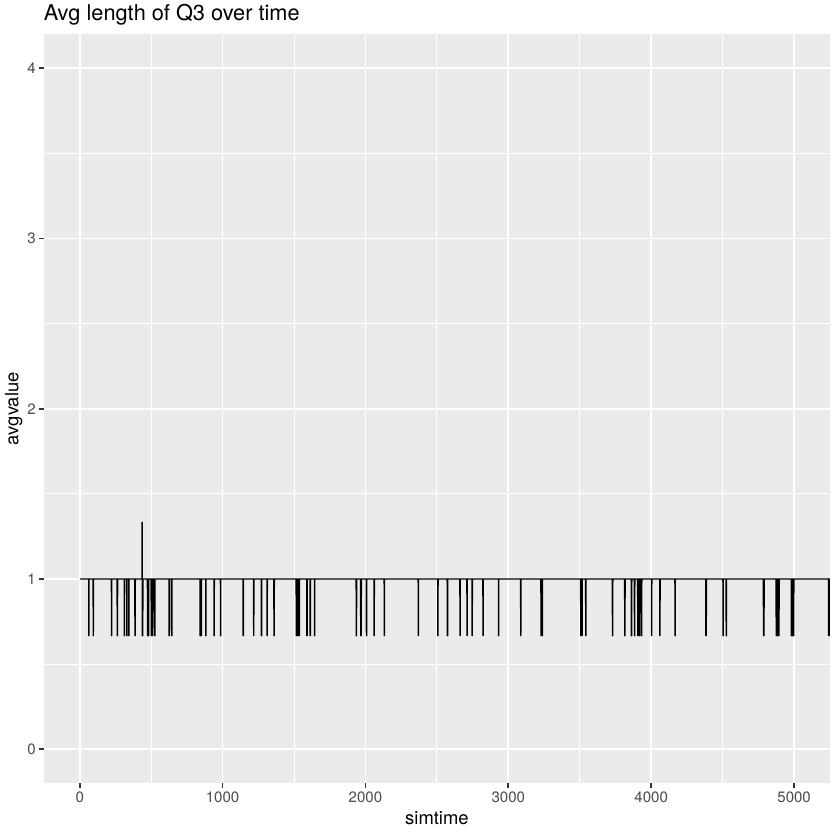
\includegraphics[width=.45\linewidth]{images/chart-q3avglength-10.png}
  \caption{p = 10s}
  \label{fig:sfig2}
\end{subfigure}
\caption{Lunghezza di \textit{Q\textsubscript{3}} per i tre rispettivi tempi di interarrivo \textit{p}}
\label{fig:fig}
\end{figure}
\newpage
%%%%% AVG LIFETIME JOBS
\begin{figure}[h!]
\begin{subfigure}{.5\textwidth}
  \centering
  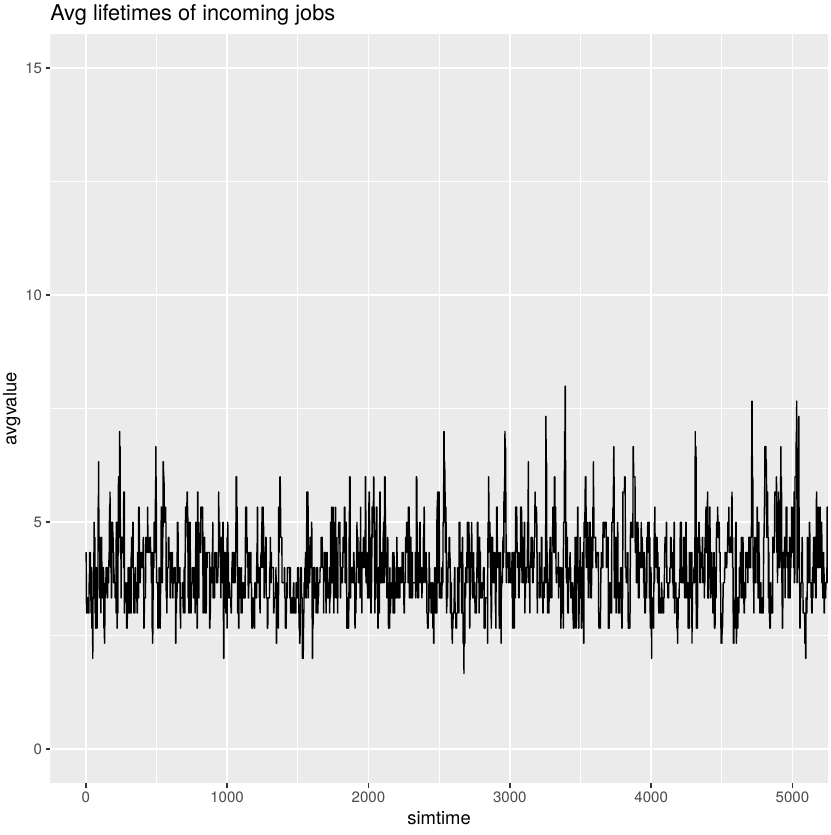
\includegraphics[width=.9\linewidth]{images/chart-avglifetime-5.png}
  \caption{p = 5s}
  \label{fig:sfig1}
\end{subfigure}%
\begin{subfigure}{.5\textwidth}
  \centering
  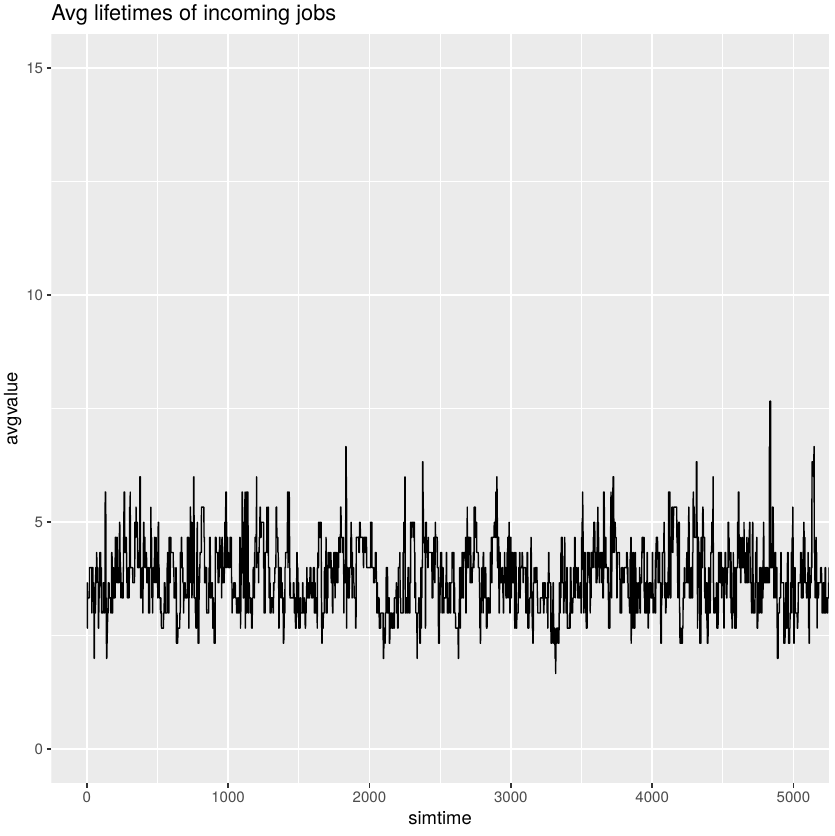
\includegraphics[width=.9\linewidth]{images/chart-avglifetime-75.png}
  \caption{p = 7.5s}
  \label{fig:sfig2}
\end{subfigure}
\begin{subfigure}{\textwidth}
  \centering
  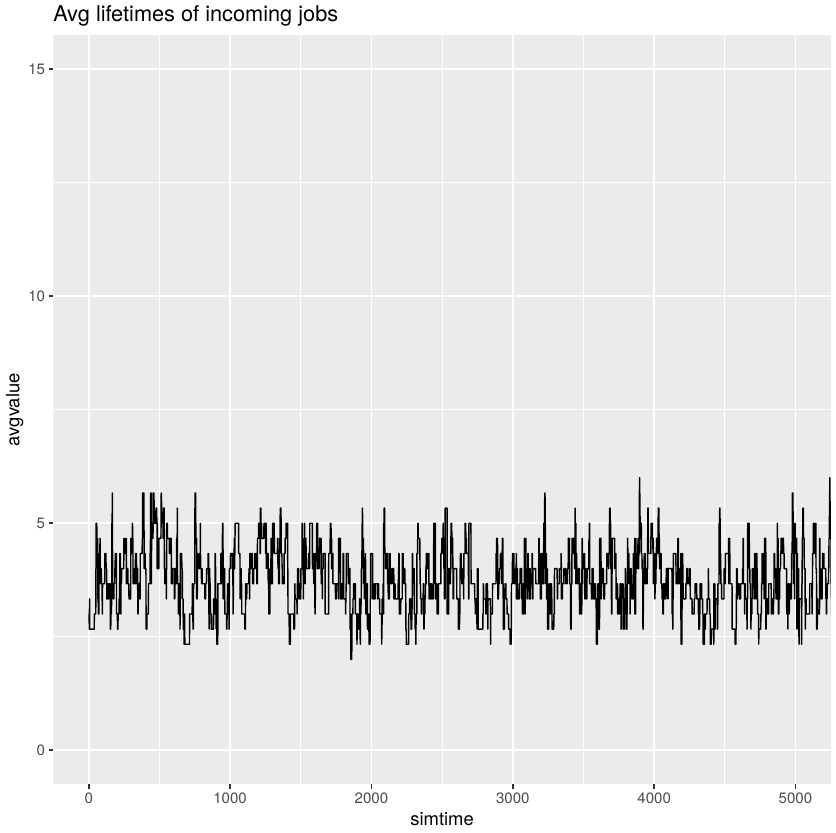
\includegraphics[width=.45\linewidth]{images/chart-avglifetime-10.png}
  \caption{p = 10s}
  \label{fig:sfig2}
\end{subfigure}
\caption{Lifetime di un job per i tre rispettivi tempi di interarrivo \textit{p}}
\label{fig:fig}
\end{figure}
\newpage
%%% NETWORK THROUGHPUT
\begin{figure}[h!]
\begin{subfigure}{.5\textwidth}
  \centering
  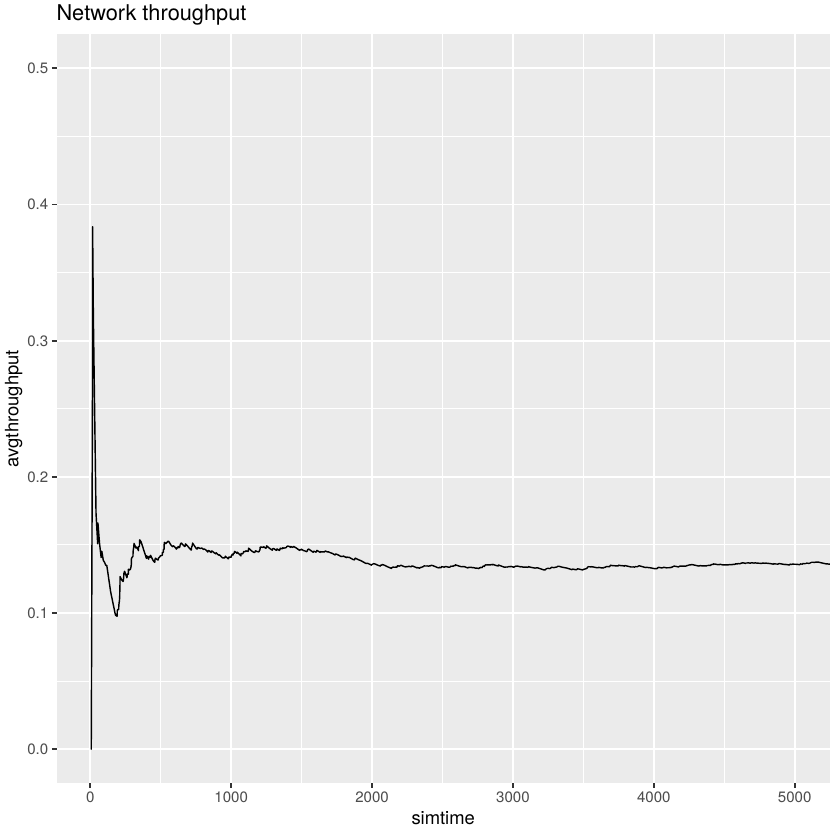
\includegraphics[width=.9\linewidth]{images/chart-throughput-5.png}
  \caption{p = 5s}
  \label{fig:sfig1}
\end{subfigure}%
\begin{subfigure}{.5\textwidth}
  \centering
  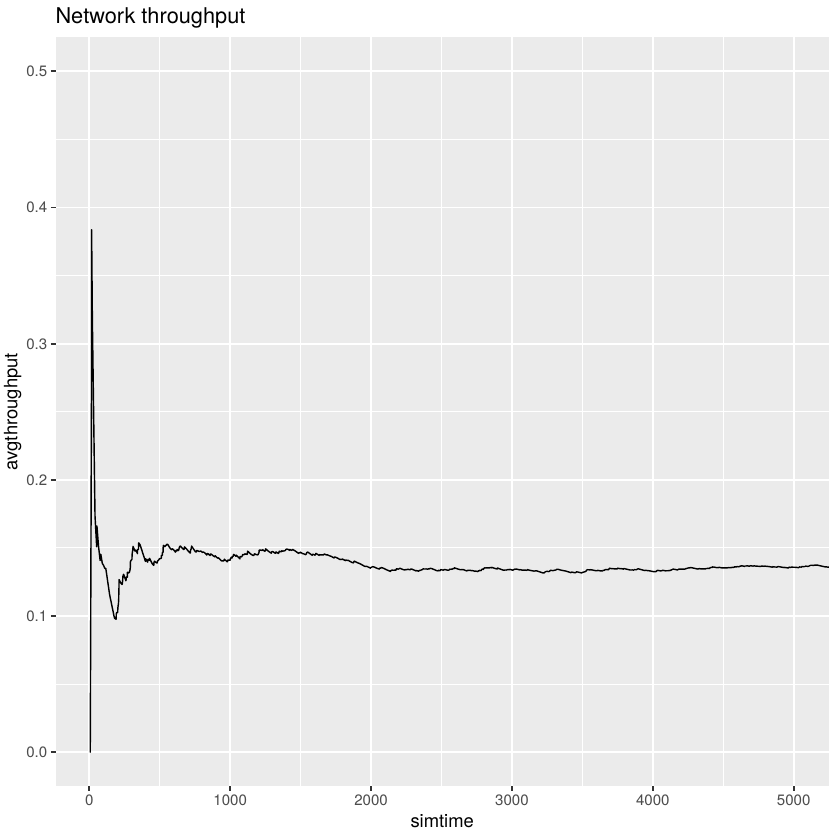
\includegraphics[width=.9\linewidth]{images/chart-throughput-75.png}
  \caption{p = 7.5s}
  \label{fig:sfig2}
\end{subfigure}
\begin{subfigure}{\textwidth}
  \centering
  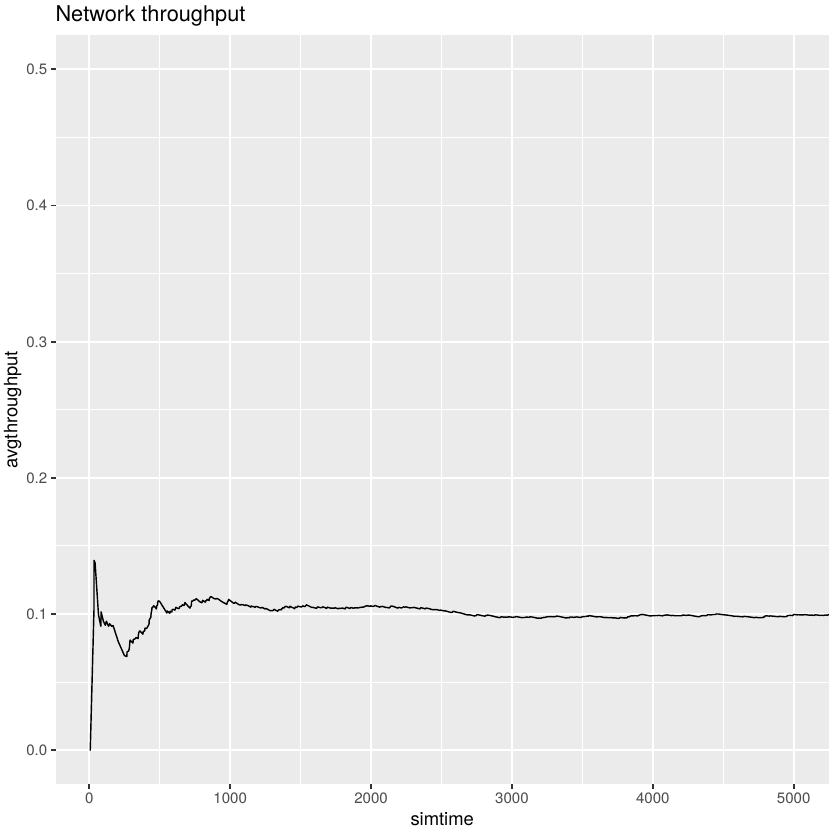
\includegraphics[width=.45\linewidth]{images/chart-throughput-10.png}
  \caption{p = 10s}
  \label{fig:sfig2}
\end{subfigure}
\caption{Throughput per i tre rispettivi tempi di interarrivo \textit{p}}
\label{fig:fig}
\end{figure}
\newpage
I grafici che descrivono la lunghezza delle code e il \textit{lifetime} medio di un job non sono informativi, mentre dal plot del throughput medio si può derivare come stima un transiente iniziale di 2000 secondi di \textit{simtime}. \newline
A questo intervallo di tempo si aggiunge un fattore del 20-30\% per evitare una sottostima. \newline
Si ottiene quindi il valore di 2600 secondi, che sono stati dati in input al simulatore OMNeT tramite l'opzione di configurazione \textit{warm-up-period} al fine di eseguire la simulazione vera e propria.

\subsection{Risultati}
La configurazione della nuova simulazione, in seguito all'eliminazione del transiente iniziale, è pensata per essere utilizzata con analisi tramite metodo batch.\newline
Prevede dunque un \textit{running time} di 600000s (circa 150h) molto più lungo del \textit{warm up} e maggiore di quello usato nella simulazione preliminare, e una sola ripetizione per ciascun parametro.\newline
L'analisi batch è eseguita dallo script \textit{analysis.R}, che calcola misure di prestazione (medie) variabili in base al numero di intervalli batch e di osservazioni per batch specificati.\newline
In particolare, l'analisi è stata effettuata per le combinazioni (numero di batch, numero di osservazioni per batch) = {(30, 40), (40, 60), (10, 200)}.\newline
Per ogni stima sono determinate media (batch), varianza e intervalli di confidenza della distribuzione t-student.
I risultati sono riportati nelle tabelle presenti nelle pagine successive.

\begin{table}[H]
    \begin{tabular}{lllll}
    \rowcolor{LightPurple}
    p & q1 length: mean & q1 length: var & q1 length: int l & q1 length: int r \\
    \rowcolor{Gray}
    5 & 0.74333 & 0.01582 & 0.70431 & 0.78235 \\
    7.5 & 0.67500 & 0.00944 & 0.64486 & 0.70514 \\
    \rowcolor{LightCyan}
    10 & 0.62167 & 0.00839 & 0.59326 & 0.65008 \\
    \rowcolor{LightPurple}
    p & q2 length: mean & q2 length: var & q2 length: int l & q2 length: int r \\
    \rowcolor{Gray}
    5 & 0.76667 & 0.02764 & 0.71510 & 0.81824 \\
    7.5 & 0.69500 & 0.01196 & 0.66107 & 0.72893 \\
    \rowcolor{LightCyan}
    10 & 0.63833 & 0.00977 & 0.60767 & 0.66899 \\
    \rowcolor{LightPurple}
    p & q3 length: mean & q3 length: var & q3 length: int l & q3 length: int r \\
    \rowcolor{Gray}
    5 & 0.77000 & 0.04217 & 0.70630 & 0.83370 \\ 
    7.5 & 0.69333 & 0.01771 & 0.65205 & 0.73461 \\
    \rowcolor{LightCyan}
    10 & 0.65000 & 0.01276 & 0.61496 & 0.68504 \\ 
    \rowcolor{LightPurple}
    p & lifetime: mean & lifetime: var & lifetime: int l & lifetime: int r \\
    \rowcolor{Gray}
    5 & 3.83960 & 0.06389 & 3.76119 & 3.91801 \\
    7.5 & 3.67062 & 0.04146 & 3.60745 & 3.73379 \\
    \rowcolor{LightCyan}
    10 & 3.62975 & 0.02790 & 3.57793 & 3.68157 \\
    \rowcolor{LightPurple}
    p & throughput: mean & throughput: var & throughput: int l & thoughput: int r \\
    \rowcolor{Gray}
    5 & 0.19764 & 0.00009 & 0.19470 & 0.20058 \\
    7.5 & 0.13377 & 0.00001 & 0.13279 & 0.13475 \\
    \rowcolor{LightCyan}
    10 & 0.09729 & 0.00004 & 0.09533 & 0.09925 \\
\end{tabular}
\caption{numbatch = 30, numobs = 40} \label{tab:tab1}
\end{table}

\begin{table}[H]
\begin{tabular}{lllll}
    \rowcolor{LightPurple}
    p & q1 length: mean & q1 length: var & q1 length: int l & q1 length: int r \\
    \rowcolor{Gray}
    5 & 0.73417 & 0.00857 & 0.70951 & 0.75883 \\ 
    7.5 & 0.66500 & 0.00689 & 0.64289 & 0.68711 \\
    \rowcolor{LightCyan}
    10 & 0.62500 & 0.00494 & 0.60628 & 0.64372 \\
    
    \rowcolor{LightPurple}
    p & q2 length: mean & q2 length: var & q2 length: int l & q2 length: int r \\
    \rowcolor{Gray}
    5 & 0.76083 & 0.01435 & 0.72892 & 0.79274 \\
    7.5 & 0.67667 & 0.00810 & 0.65269 & 0.70065 \\
    \rowcolor{LightCyan}
    10 & 0.63750 & 0.00616 & 0.61659 & 0.65841 \\
    
    \rowcolor{LightPurple}
    p & q3 length: mean & q3 length: var & q3 length: int l & q3 length: int r \\
    \rowcolor{Gray}
    5 & 0.77083 & 0.01733 & 0.73576 & 0.80590 \\
    7.5 & 0.66500 & 0.00928 & 0.63934 & 0.69066 \\
    \rowcolor{LightCyan}
    10 & 0.63000 & 0.00609 & 0.60921 & 0.65079 \\
    
    \rowcolor{LightPurple}
    p & lifetime: mean & lifetime: var & lifetime: int l & lifetime: int r \\
    \rowcolor{Gray}
    5 & 3.80783 & 0.03773 & 3.75608 & 3.85958 \\
    7.5 & 3.68995 & 0.01755 & 3.65466 & 3.72524 \\
    \rowcolor{LightCyan}
    10 & 3.63671 & 0.01900 & 3.59999 & 3.67343 \\
    
    \rowcolor{LightPurple}
    p & throughput: mean & throughput: var & throughput: int l & thoughput: int r \\ 
    \rowcolor{Gray}
    5 & 0.19933 & 0.00004 & 0.19765 & 0.20101 \\
    7.5 & 0.13324 & 0.00005 & 0.13240 & 0.13408 \\
    \rowcolor{LightCyan}
    10 & 0.09750 & 0.00002 & 0.09631 & 0.09869 \\
\end{tabular}
\caption{numbatch = 40, numobs = 60} \label{tab:tab1}
\end{table}

\begin{table}[H]
\begin{tabular}{lllll}
    \rowcolor{LightPurple}
    p & q1 length: mean & q1 length: var & q1 length: int l & q1 length: int r \\
    \rowcolor{Gray}
    5 & 0.73300 & 0.00247 & 0.70419 & 0.76181 \\
    7.5 & 0.66000 & 0.00156 & 0.63710 & 0.68290 \\
    \rowcolor{LightCyan}
    10 & 0.62800 & 0.00100 & 0.60967 & 0.64633  \\
    
    \rowcolor{LightPurple}
    p & q2 length: mean & q2 length: var & q2 length: int l & q2 length: int r \\
    \rowcolor{Gray}
    5 & 0.76000 & 0.00549 & 0.71705 & 0.80295 \\
    7.5 & 0.67300 & 0.00225 & 0.64550 & 0.70050 \\
    \rowcolor{LightCyan}
    10 & 0.64100 & 0.00074 & 0.62523 & 0.65677 \\
    
    \rowcolor{LightPurple}
    p & q3 length: mean & q3 length: var & q3 length: int l & q3 length: int r \\
    \rowcolor{Gray}
    5 & 0.77900 & 0.01012 & 0.72069 & 0.83731  \\
    7.5 & 0.67800 & 0.00393 & 0.64166 & 0.71434 \\
    \rowcolor{LightCyan}
    10 & 0.63100 & 0.00399 & 0.59438 & 0.66762 \\
    
    \rowcolor{LightPurple}
    p & lifetime: mean & lifetime: var & lifetime: int l & lifetime: int r \\
    \rowcolor{Gray}
    5 & 3.80277 & 0.01357 & 3.73524 & 3.87030  \\
    7.5 & 3.69224 & 0.00295 & 3.66076 & 3.72372 \\
    \rowcolor{LightCyan}
    10 & 3.63064 & 0.00268 & 3.60063 & 3.66065 \\
    
    \rowcolor{LightPurple}
    p & throughput: mean & throughput: var & throughput: int l & thoughput: int r \\ 
    \rowcolor{Gray}
    5 & 0.19866 & 0.00002 & 0.19607 & 0.20125 \\
    7.5 & 0.13312 & 0.00005 & 0.13129 & 0.13495 \\
    \rowcolor{LightCyan}
    10 & 0.09734 & 0.00001 & 0.09551 & 0.09917 \\
    
\end{tabular}
\caption{numbatch = 10, numobs = 200} \label{tab:tab1}
\end{table}

\newpage

\section{Conclusioni}
Nel progetto qui presentato si è svolta una simulazione di un sistema a tre code che modellano una rete opportunistica. \newline 
Il comportamento del modello è stato implementato in C++ attraverso il simulatore OMNeT++ e l'analisi statistica effettuata in R verteva su tre misure di prestazione, numero medio di utenti in coda, tempo medio di risposta, throughput medio del sistema. \newline
Una prima analisi ha consentito di individuare il transiente iniziale, non interessante ai fini statistici. 
Una volta eliminato il transiente, attraverso l'analisi con metodo batch si sono stimate infine media, varianze e intervalli di confidenza.

\begin{thebibliography}{90}

\bibitem{K} A. Al-Hanbali, R. de Haan, R. J. Boucherie, J. van Ommeren, \textit{A Tandem Queueing Model for Delay Analysis in Disconnected Ad Hoc Networks.}
\bibitem{K} \textit{OMNeT++ Documentation}, https://docs.omnetpp.org/.
\bibitem{K} \textit{OMNeT++ User Guide}, https://doc.omnetpp.org/omnetpp/UserGuide.pdf.
\bibitem{K} \textit{OMNeT++ Simulation Manual}, https://doc.omnetpp.org/omnetpp/manual/.
\bibitem{K} Emmanuel Paradis, \textit{R for Beginners}, https://cran.r-project.org/doc/contrib/Paradis-rdebuts\_en.pdf.
\end{thebibliography}

\end{document}